\documentclass[12pt,a4paper,oneside]{article}

\usepackage[pdftex,
            pdfauthor={Albert Zak},
            pdftitle={Design, Implementation and Evaluation of a Hands-off Build Pipeline for Erlang/OTP Projects},
            pdfsubject={Bachelor's Thesis},
            hidelinks,
            driverfallback=hypertex]{hyperref}
\usepackage[utf8]{inputenc}
\usepackage[T1]{fontenc}
\usepackage{geometry}
\usepackage{bookmark}
\usepackage{listings}
\usepackage[inline]{enumitem}
\usepackage{subcaption}
\usepackage{tabularx}
\usepackage{hhline}
\usepackage{algpseudocode}
\usepackage{tikz}
\usetikzlibrary{trees,arrows,fit,positioning,shapes.geometric}
\PassOptionsToPackage{usenames,dvipsnames,svgnames,table}{xcolor}
\usepackage{xcolor-solarized}
\usepackage{gitdags}
\usepackage[singlespacing]{setspace}
\usepackage[acronym,nopostdot,style=super,nonumberlist,nogroupskip]{glossaries}
\usepackage{fancyhdr}

\pagestyle{fancy}
\fancyhf{}
\cfoot{\thepage}
\renewcommand{\headrulewidth}{0pt}

\makeglossaries{}
\newacronym{mfa}{MF[A]}{Module, Function, and List of Arguments}


\lstset{
  language=erlang,
  numbers=left,
  numberstyle=\small\color{lightgray},
  basicstyle=\ttfamily,
  frame=tb
}

\pdfpageheight=297mm
\pdfpagewidth=210mm
\geometry{a4paper, left=30mm, right=25mm, top=30mm, bottom=30mm}

\begin{document}

\cleardoublepage{}

\chapter*{Abstract}

The Erlang/OTP Release process requires manual interaction at many steps. Previous work on automating Erlang/OTP Release generation has addressed parts of the process by abstracting the low-level mechanics of the build step, but tasks such as versioning, writing upgrade instructions, and handling artifacts were left to the developer. This thesis proposes  the design of a build tool that trades customizability for hands-off operation as part of a Continuous Integration (CI) pipeline.


\tableofcontents{}

\renewcommand{\glsnamefont}[1]{\textbf{#1}}
\doublespacing
\printglossary[nonumberlist,type=\acronymtype]
\singlespacing

\section{Introduction}

The contribution of this work is a tool that automates the steps required to generate deployable artifacts of Erlang/\acrshort{otp} projects using a single command that runs without user interaction.
This section explains relevant terminology and shows where manual interaction is required to generate \acrshort{otp} Releases. An overview of existing tooling and how they build on top of each other follows.

\subsection{Erlang/OTP}

Erlang is a programming language for building concurrent, distributed systems with high availability requirements. Initially designed by Ericsson for telephone exchanges, it has been embraced by industries with similar needs: finance, gaming, betting, messaging, middleware, and databases. Development of Erlang took place starting in 1986 at the Ericsson Computer Science Laboratory, and in 1998 Erlang was released as Open Source.~\cite{armstrong2007history}

\acrshort{otp} stands for \acrlong{otp}, and is a combination of library applications, design patterns, conventions, and documentation. Erlang is almost always used in conjunction with \acrshort{otp}, hence the name Erlang/\acrshort{otp}.~\cite{ferd}

The language is often described as functional, although it is not strictly side-effect free or referentially transparent. Erlang compiles to bytecode, which is executed by a \acrfull{vm}. The current Erlang \acrshort{vm} – the \acrshort{beam}, short for \acrlong{beam} – is written in C and supports various machine architectures. Multiple languages that compile to \acrshort{beam} bytecode have been created, most famously \emph{Elixir} and \emph{Lisp Flavored Erlang}. Actor model processes are the language's concurrency primitives: Functions can be spawned to create lightweight \acrshort{beam} processes. They are different from \acrshort{os} processes or threads, being preemptively scheduled by the \acrshort{beam}. Erlang/\acrshort{otp} systems commonly ``run millions of processes simultaneously [with each one taking] less than a kilobyte of space.''~\cite{larson}

\paragraph{\acrshort{otp} Applications.}
Erlang code is constructed out of functions defined within \mbox{\emph{module}} files bearing an \lstinline|*.erl| extension. \emph{\acrshort{otp} Applications} group related modules into reusable units to provide well-defined start and stop semantics, including an \emph{application resource file} (\lstinline|*.app|) containing additional metadata such as a version string and a list of other applications that this application depends on, and which need to be started beforehand. Every application has a dependency on at least \lstinline|kernel| and \lstinline|stdlib|, and both must be specified in the application resource file.~\cite{doc:otp}

\acrshort{otp} also enforces a certain directory structure for applications.~\cite{logan:otp}

\paragraph{\acrshort{otp} Releases.} Whole projects consisting of multiple applications are packaged and deployed as \acrshort{otp} Releases. They are described by a release resource (\lstinline|*.rel|) file, which specifies additional metadata, such as a version string for the entire release, the included version of the \acrfull{erts}, and a list of applications with their respective version strings that comprise the release.

From this release resource file, various tools can be used to create a boot script and assemble the release into a single compressed tarball (\lstinline|*.tar.gz|) package.~\cite{doc:otp} A packaged release contains everything necessary to bootstrap an \emph{embedded target system} on another machine, also called a \emph{node}. Depending on the tool used to generate the release, it may include additional convenience scripts to upgrade or inspect the target system.

\paragraph{\acrlong{dsu}.} A core feature of Erlang is its support for \acrfull{dsu}, also referred to as on-the-fly upgrading, or hot code loading. The \acrshort{beam} keeps up to two versions of a module loaded in memory, and both versions of the code may run side by side.~\cite{cesarini:otp} \acrshort{otp} provides generic \emph{behaviours} that \emph{callback modules} can implement to normalize start, stop and upgrade semantics, among others.~\cite{doc:otp} Erlang systems constructed according to \acrshort{otp} patterns, grouped into \acrshort{otp} Applications, and packaged as \acrshort{otp} Releases enjoy additional support for \acrshort{dsu} via instruction files: \acrshort{appup}s and \acrshort{relup}s.

First, there are high-level, often hand-written \acrfull{appup} files, one for each \acrshort{otp} Application. These files are fed into release generation tools where they are translated and combined into a single low-level \acrshort{relup} file, thus making a given release \acrshort{dsu}-capable.~\cite{doc:otp} The \acrshort{relup} file contains instructions on how to upgrade a node running a previous version. A single release package can include one \acrshort{relup} file which may know how to upgrade from multiple previous releases. These files also contain instructions on how to downgrade to the previous version in case the upgrade fails.~\cite{doc:otp}

\subsection{Problem}\label{sec:problem} Most existing release generation tools require manual interaction at various steps, and are generally not trivial to set up and use out of the box in a non-interactive build environment, such as a \acrfull{ci} pipeline. Additionally, there are some pitfalls when developers assemble releases on, for example, their \emph{macOS} development machines and then attempt to start them on \emph{Linux} in production~\cite{cesarini:otp}: This fails with a non-obvious error. To generate a \acrshort{dsu}-capable \acrshort{otp} Release, a developer needs to manually write \acrshort{appup} files and increment version numbers for all changed applications. The \acrshort{otp} Release resource file has an additional, separate version number that needs to be updated between commits to be able to perform \acrshort{dsu}. Then, to generate upgrade instructions, previous releases need to be fetched and unpacked. Lastly, the developer has to invoke various commands to assemble the final release package tarball.~\cite{ferd}

This process is tedious to perform manually, and impedes frequent deployment of small changes. Likewise, complex code changes are more likely to fail when applied via \acrshort{dsu}.~\cite{hicks} The unfortunate consequence is that developers are discouraged from using Erlang's \acrshort{dsu} capabilities unless absolutely necessary.~\cite{ferd}

\subsection{Contribution}

This work contributes design, implementation and evaluation of a \acrshort{dsu}-capable release generation tool for Erlang/\acrshort{otp} projects named \emph{BeamUp}. Its aim is to run without user interaction and to require as little configuration as possible.

\paragraph{Goal.} The goal is to develop a prototype implementation that produces \acrshort{otp} release packages. The tool should be easy to setup on major hosted \acrfull{ci} platforms~\cite{dig2016usage}, and integrate with the Git \acrfull{vcs}~\cite{sink2011version} to use commit hashes as version strings, instead of requiring the developer to hand-increment version numbers.~\cite{maste2016} It must handle generating \acrshort{dsu} instructions, as well as assembling and storing \acrshort{otp} Releases in a completely automated, hands-off way so that the tool may be used as part of a \acrshort{ci} pipeline.

\paragraph{Method.} The thesis describes in detail the architectural and design decisions made while iteratively implementing said build tool. The prototype is evaluated for correctness and run time performance on six hosted \acrshort{ci} platforms that provide a free tier: \emph{CircleCI, Codeship, Semaphore, Shippable, Travis CI,} and \emph{Wercker}. Finally, the work discusses limitations and advantages of the proposed tool.

\cleardoublepage
\subsection{State of the Art}\label{sec:sota}

The proposed tool, \emph{BeamUp}, relies on several layers of existing tooling, as visualized in figure~\ref{fig:tools}. At the lowest level, Erlang/\acrshort{otp} ships with the \acrfull{sasl} that include the two basic building blocks for \acrshort{dsu} support: \lstinline|systools| provides low-level functions for \emph{offline} release generation, and \lstinline|release_handler| is used to perform an \emph{online} hot-upgrade of a running node.~\cite{doc:otp}
Elixir projects are built with \lstinline|mix| (not pictured) and releases are generated with \lstinline|distillery|~\cite{distillery}, which handles generation of upgrade instructions itself, and directly interacts with \lstinline|systools|. Erlang projects, however, need more coaxing: Modules and dependencies are compiled with \lstinline|rebar3|, \acrfull{appup} files are generated on a best-effort basis by comparing \acrshort{beam} bytecode via a plugin to \lstinline|rebar3|~\cite{rebar3appup}, while release assembly is done by another intermediary tool, \lstinline|relx|~\cite{loder2016production}.

\vspace{2cm}
\begin{figure}[h]
  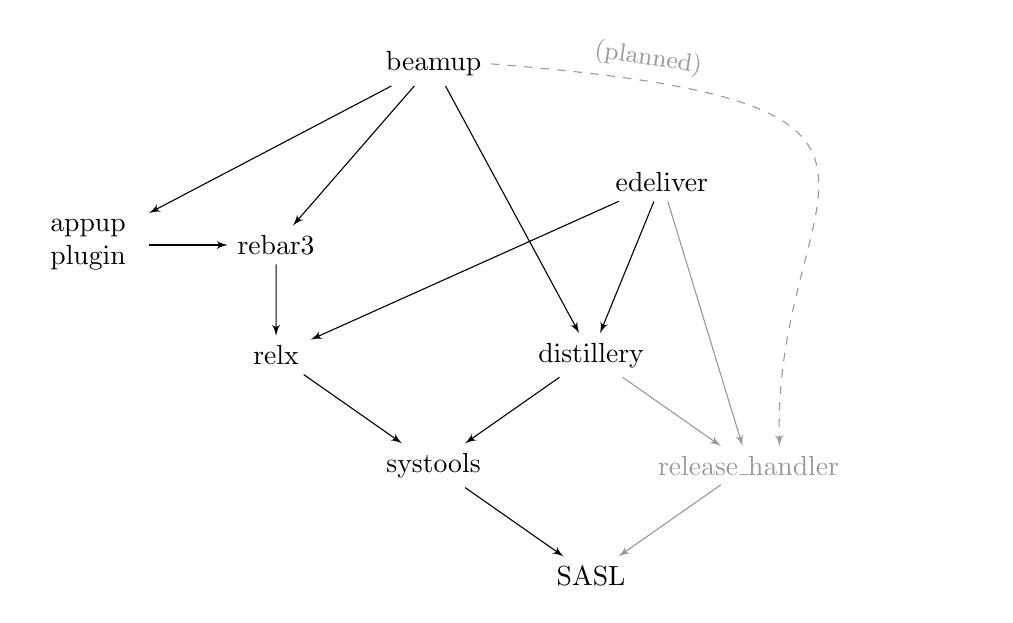
\begin{tikzpicture}[sibling distance=40mm,
    level distance=14mm,edge from parent,>=latex']
    \tikzstyle{edge from parent}=[draw,<-]
    \node (edeliver) at (0.9, 5) {\lstinline|edeliver|};
    \node (beamup) at (-2, 6.5) {\lstinline|beamup|};

    \node {\lstinline|SASL|} [grow'=up] {
      child {node {\lstinline|systools|}
        child {node (relx) {\lstinline|relx|}
          child {node (rebar3) {\lstinline|rebar3|}}}
        child {node (distillery) {\lstinline|distillery|}}}
      child {node (release_handler) [text=black!40] {\lstinline|release_handler|} edge from parent[draw=black!40]}
    };

    \node (appup) [left=10mm of rebar3,text centered,text width=13mm] {\lstinline|appup| \lstinline|plugin|};

    \draw[->] (appup) -- (rebar3);

    \draw[->] (edeliver) -- (distillery);
    \draw[->] (edeliver) -- (relx);
    \draw[->,draw=black!40] (edeliver) -- (release_handler);
    \draw[->,draw=black!40] (distillery) -- (release_handler);

    \draw[->] (beamup) -- (distillery);
    \draw[->] (beamup) -- (rebar3);
    \draw[->] (beamup) -- (appup);
    \draw[->,dashed,draw=black!40] (beamup.east) .. controls (5,6) and (2.3,5) .. node[very near start,sloped,above,text=black!40] {\small{(planned)}} (release_handler.32);

  \end{tikzpicture}
  \caption{Dependencies between selected tools to create and handle releases.}\label{fig:tools}
\end{figure}

\cleardoublepage
\section{Related Work}\label{sec:related_work}

There have been several attempts to automate Erlang/\acrshort{otp} release generation.

\emph{Sinan}~\cite{sinan} was a widely used tool to simplify assembling releases, but did not automate generation of \acrshort{appup}s. The project is deprecated since 2012.

\emph{Knit}~\cite{davis:knit,davis:talk} aimed for simple operation; requiring just one command to generate a \acrshort{dsu}-capable release from previous packages. Knit relied on the build tool \lstinline|rebar|, which – unlike its successor \lstinline|rebar3| - included an algorithm similar to~\cite{rebar3appup} for generating \acrshort{appup}s. Knit optionally took metadata hints from the developer via \emph{module attributes} to guide \acrshort{appup} generation. The project was last updated in 2014 and appears to be abandoned.

\emph{Relflow}~\cite{relflow} integrates with the Git \acrshort{vcs} and automatically versions releases by rewriting the the \lstinline|rebar3| config file. It uses its own \acrshort{appup} generation algorithm that relies on Git to detect what modules have changed between versions.

\emph{Tetrapak}~\cite{tetrapak} is an alternative release assembling tool that outputs artifacts as Debian packages. It too supports configurable automated versioning from \acrshort{vcs} commits, but has no support for \acrshort{dsu}.

\emph{Edeliver}~\cite{edeliver,talk:edeliver} shares very similar goals to the proposed tool. It supports Erlang and Elixir projects, coaxing any of the following tools used on a project: \lstinline|rebar|, \lstinline|relx|, \lstinline|exrm|, or \lstinline|distillery|. It generates \acrshort{dsu}-capable releases with configurable auto-generated version strings. To provide a repeatable build environment, Edeliver opens a \acrfull{ssh} tunnel to a separate build host and assembles the release remotely. Written in \lstinline|bash|, it has no additional dependencies. The tool alo handles deployment via \acrshort{ssh}, including remotely performing \acrshort{dsu}.

A different approach to release assembling relies on \emph{Nix}, a general-purpose package manager borrowing ideas from functional programming: immutability, pure functions, and referential transparency.~\cite{nix1} Its artifacts are identified via cryptographic hashes of all inputs used to build them. Nix provides repeatable environments to build packages inside, similar to what containers are used for in this work, but with stronger determinism. Nix forms the base of \emph{NixOS}~\cite{nixos}, a full-featured Linux distribution where almost all components are controlled by Nix via symbolic links.

Previous work by~\cite{erlangnix} allows dependencies of Erlang/\acrshort{otp} projects to be managed via Nix, relying on \cite{hex2nix} to provide Nix metadata, called \emph{Expressions}, for most of the Erlang and Elixir packages hosted on \lstinline|hex.pm|, the primary package repository of the Erlang/\acrshort{otp} ecosystem. Lastly,~\cite{erlangnix2}~presents a pipeline to deploy Erlang/\acrshort{otp} projects using Nix.

\section{Implementation}

\subsection{Launcher} The main point of entry to the \acrshort{cli} build tool is the \emph{launcher} executable. Acting as the starting point for all invocations, it is implemented as a \lstinline|bash| script mainly wrapping the \emph{Docker} client. To provide a repeatable build environment, the launcher prefers to start a well-known container to run the given command in. If, however, the launcher is invoked as part of an already-running \acrshort{ci} container, it is not possible to start a new one. Thus, the launcher first has to detect whether it is able to start containers. In case it is able to, the launcher has to pull the correct image for the host's machine architecture in combination with the requested Erlang/OTP version, set up volume mounts and environment variables, and invoke the Docker client to start the container. If the launcher is already running inside a container, the responsibility is reduced to passing through the given arguments to the \emph{container entrypoint}. The following paragraphs describe how each component of the launch sequence is implemented.

\begin{figure}[h]
  \centering
  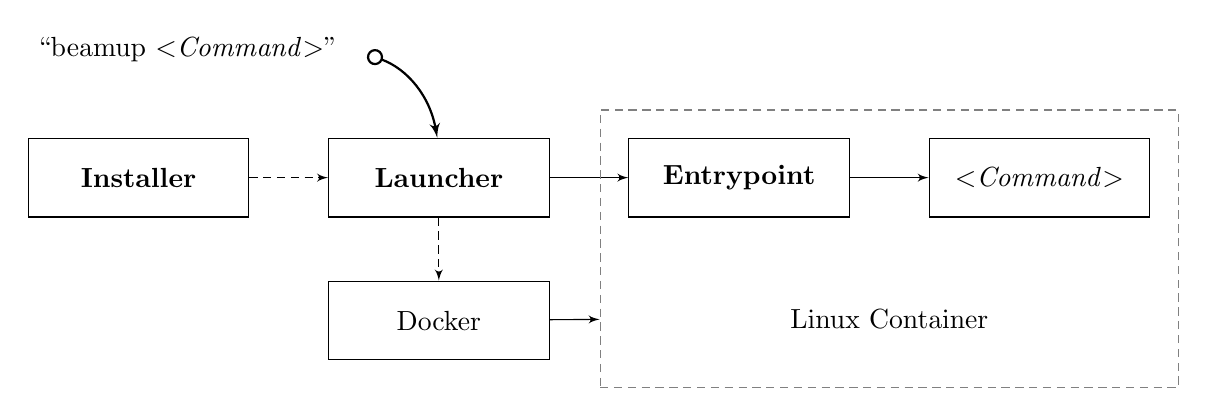
\begin{tikzpicture}[>=latex']
    \tikzset{block/.style={
      draw,
      rectangle,
      align=center,
      minimum width=2.8cm,
      minimum height=1cm
    }};

    \node [block] (installer) {\textbf{Installer}};
    \node [block, right=1cm of installer] (launcher) {\textbf{Launcher}};
    \node [block, right=1cm of launcher] (entrypoint) {\textbf{Entrypoint}};
    \node [block, right=1cm of entrypoint] (command) {$<$\emph{Command}$>$};
    \node [block, below=0.8cm of launcher] (docker) {Docker};

    \node [inner sep=0pt,
      yshift=-1.8cm,
      minimum height=0.6cm,
      fit={(entrypoint) (command)},
      label=center:Linux Container] (container) {};

    \node [
      above left=1cm and -0.5cm of launcher,
      label=left:\text{``\lstinline|beamup| $<$\emph{Command}$>$}''] (start) {};

    \path[draw,->] (launcher) edge (entrypoint)
      (entrypoint) edge (command);

    \path[densely dashed,->] (installer) edge (launcher)
      (launcher) edge (docker);

    \path[draw,o->,thick] (start) edge[bend left] (launcher);

    \node [draw=black!50, densely dashed, fit={
      (entrypoint) (command) (container)
    }, inner sep=10pt] (container_box) {};

    \path[draw,->] (docker) edge (container -|container_box.west);

  \end{tikzpicture}
  \caption{Execution sequence of build pipeline components.}
\end{figure}

\paragraph{Installation.} The recommended way to install the \acrshort{cli} tool is by downloading a \lstinline|bash| script and piping it to the shell. This pattern is informally known as ``curl pipe sh'', and while common because of its simplicity, brings security implications which are discussed in section~\ref{sec:curlpipesh}. A Content Delivery Network, \emph{Cloudflare}, is used to ensure the installer script is exclusively served with \acrfull{tls}.

\begin{lstlisting}[
  label={lst:curlpipesh},
  caption={CLI tool installation command}
]
curl https://get.beamup.io/install | /bin/sh
\end{lstlisting}

When the installer detects it is being executed inside an interactive terminal session, it pauses for a few seconds to give the user a chance to abort installation. Next, the installer clones the \acrshort{cli} repository to the \lstinline|~/.beamup| folder of the current user's home directory. Note that cloning a repository keeps file permissions intact, including the executable bits that are set on the main \acrshort{cli} launcher script. At no point are super user permissions needed, consequently the installer first attempts to create a symbolic link to the \acrshort{cli} launcher, and optionally falls back to displaying instructions on how to add the just-installed tool to the executable path. Finally, to make sure that the installation was successful, the launcher is invoked for a self-test.

\paragraph{Self-update.} Because the \acrshort{cli} tool is little more than a local clone of a remote repository, distributing and installing updates to the tool itself becomes as trivial as pulling changes from the remote. A convenience wrapper is provided.

\paragraph{Project scaffolding.} To quickly create basic folder structure and files for new projects in various \acrshort{beam} languages, the \acrshort{cli} provides a convenience command.

\paragraph{Transparent container invocation.} All commands first go through the launcher, which must set up a container to run the given command in; or run the command directly. Many \acrshort{ci} platforms confine the whole build process to a container that has already been set up and started, allowing only limited configuration of the container's parameters. Since it is not always possible to start a clean container, the tool must be able to either operate inside an already-running \acrshort{ci} container, or transparently start a new container and pass control inside.

First, the launcher  attempts to detect where it is being called from by parsing the \emph{control group (cgroup)} file. While detection in this way is widespread, it is not recommended, since it relies on an implementation detail of the container runtime. However, work to add container introspection capabilities is ongoing\footnote{\url{https://github.com/moby/moby/pull/26331}}. To provide a temporary solution until an interface is finalized and widely deployed, the tool checks for artifacts of common container runtime implementations in the \emph{cgroup} file: \emph{Docker}, \emph{\acrfull{lxc}}, and \emph{\acrfull{aws} \acrfull{ecs}}. If the tool is being run inside a container, execution is simply passed to the \emph{container entrypoint} along with all arguments under the assumption that the container's environment is sufficiently correct, i.e.~has the correct version of Erlang/OTP installed.

\paragraph{Determining the base image.} When the launcher determines that it is able to start a container to run the build in, i.e.~the tool is being invoked inside a \acrshort{vm} or on bare metal, it needs to consider the following two attributes to determine which image to instantiate a container from:
\begin{enumerate*}[label=(\roman*)]
  \item The requested version of Erlang/OTP, read from an environment variable, and
  \item the host's machine architecture.
\end{enumerate*}

Concerning the machine architecture, official builds of Erlang/OTP for various architectures are provided on the \emph{Docker Hub}. Such images are available under the namespace of the respective architecture identifiers as used by the \emph{Go} programming language. A challenge lies in reliably normalizing the machine architecture as reported by \lstinline|uname -m|. Note that since version \emph{17.06 Docker} implicitly pulls images for the correct architecture. However, because the tool is designed to support \emph{Docker} down to version \emph{1.12}, the launcher has to manually determine the architecture and map it to an image namespace identifier using the normalization given in table~\ref{table:architectures}.

\begin{table}
  \setlength{\tabcolsep}{10pt}
  \centering
  \begin{tabular}{ r l }
    Output of \lstinline|uname -m| & Identifier \\
    \hline
    \lstinline|arm arm32 armv7 armv7l armhfp| & \lstinline|arm32v7| \\
    \lstinline|arm64 armv8 armv8b armv8l aarch64 aarch64_be| & \lstinline|arm64v8| \\
    \lstinline|i386 i686 i686-64 i686-AT386| & \lstinline|i386| \\
    \lstinline|s390x s390| & \lstinline|s390x| \\
    \lstinline|ppc ppc64 ppcle ppc64le| & \lstinline|ppc64le| \\
    \emph{other} & \lstinline|amd64| \\
  \end{tabular}
  \caption{Mapping between reported machine architecture and image identifier.}\label{table:architectures}
\end{table}

Note that support for other \acrshort{beam} languages such as Elixir is handled within the \emph{container entrypoint}, and it is sufficient to pull an image containing just the Erlang/OTP runtime at this point. Additionally, there are currently no official images of Elixir available for all machine architectures supported by the Erlang/OTP images.


\paragraph{Project mount.} Clearly, the build tool needs access to the directory containing the Erlang/OTP project to be built. The launcher is meant to be invoked inside that directory, and derives the project's name from the name of the current working directory. The build tools must not permanently alter any files of the original project folder on the host as doing so may interfere with other parts of the build pipeline. To guarantee that the project files remain unmodified, the current working directory is mounted as a read-only volume.

\begin{table}[h]
  \setlength{\tabcolsep}{10pt}
  \centering
  \begin{tabular}{ l c l }
    Host & & Container \\
    \hline
    Current working directory &
      $\Longrightarrow$ &
      Project directory \\
    Combined cache directory &
      $\Longleftrightarrow$ &
      $<$\emph{Various cache directories}$>$ \\
    RAM disk or temporary directory &
      $\Longleftrightarrow$ &
      Temporary directory \\
  \end{tabular}
  \caption{Container volume mounts.}
\end{table}

\paragraph{Virtual RAM disk.} The run time of the build tool is bound by performance of the filesystem and storage media. Additionally, building upgrade releases causes the entire project folder to be temporarily duplicated for each previous release.
If supported by the \emph{Docker} client, the container's \lstinline|/tmp| directory is mounted as a temporary filesystem (\emph{tmpfs}) on the host's \acrshort{ram}. In case the size of the temporary file system grows beyond the available \acrshort{ram}, the host \acrshort{os} transparently falls back to consuming swap space.


\paragraph{Cache mount.} Minimizing build run time is crucial for a pleasant \acrlong{ci} workflow. Many \acrshort{ci} platforms offer a way to cache the contents of certain folders between build runs. A number of cache folders of the container are bind-mounted to a single cache path in the host user's home directory. Combining the cache paths into one folder on the host makes it trivial to setup caching, as instead of having to configure multiple, possibly changing paths for each tool separately, it is sufficient to cache just one folder. Currently, the host cache folder combines bind mounts of the following locations inside the container:
\begin{itemize}
  \item Compiled artifacts and dependencies of the build tool itself;
  \item Dependency cache directories of the build tools \lstinline|rebar3| and \lstinline|mix|;
  \item Erlang and Elixir interactive shell history files;
  \item Precompiled, downloaded, and extracted Elixir release.
\end{itemize}
Note that if the launcher is unable to start a container, caching would have to be set up explicitly for each location.

\paragraph{Environment variables.} All configuration for the tool is provided via environment variables, instead of files or interactive menus. Most \acrlong{ci} platforms provide a straightforward way to configure environment variables for the build pipeline, and many offer additional facilities to encrypt or otherwise store environment variables in a secure way. The launcher reads various environment variables and other parameters of the host, applies transformations, and passes configuration on to the \emph{container entrypoint}, again via environment variables.

\begin{table}[h]
  \setlength{\tabcolsep}{10pt}
  \centering
  \begin{tabularx}{\textwidth}{l X X}
    Host & Launcher & Container entrypoint \\
    \hline
    \emph{Working directory} &
      Passed as \lstinline|PROJECT_DIR| \newline
      either as-is or with container path of mount point &
      Passed through \\
    \hline
    \lstinline|ERLANG_VERSION| &
      Used to determine \newline
      image identifier &
      Validated against \newline
      currently installed version \\
    \hline
    \lstinline|ELIXIR_VERSION| &
      Passed through &
      Used to validate and/or \newline
      install Elixir \\
    \hline
    --- &
      \lstinline|TERM| set to \lstinline|dumb| &
      Passed through \\
    \hline
    --- &
      Contents read from global gitignore
      file and passed on as \lstinline|GLOBAL_GITIGNORE| &
      Contents written to \newline
      container's global \newline
      \emph{gitignore} file \\
    \hline
    \lstinline|STORE| & Passed through & Passed through \\
    \hline
    \lstinline|STORE_SECRET| & Passed through & Passed through \\
    \hline
    \lstinline|DEBUG| & Passed through & Passed through \\
  \end{tabularx}
  \caption{Transformation of environment variables between host and container.}\label{table:envvars}
\end{table}

Since the tool must run without interactivity, the launcher exports the \lstinline|TERM| variable set to ``\lstinline|dumb|''. Additionally, the contents of the host's global \emph{gitignore} file are read into an environment variable, passed into the container entrypoint, to be written out again. This avoids situations where host sees the working tree as clean, while the builder refuses to run because files may be present that would be ignored by the host, but not by the builder. Note that neither the architecture of the host, nor the architecture part of the image identifier are passed into the container, as the builder internally retrieves the system architecture string as reported by Erlang/OTP, which differs from the identifier used at the launcher stage. Lastly, authentification credentials for the store are passed through, as is a flag to enable verbose debug output. See table~\ref{table:envvars} for an overview of how various parts of the build pipeline use environment variables to pass and transform configuration.

\paragraph{Container entrypoint.} As stated above, the \acrshort{cli} may be launched inside an already-running container, or start a clean container. In any case, the \emph{container entrypoint} is a \lstinline|bash| script that is always executed inside a container. Yet it may only make minimal assumptions about its environment since the container may have been set up already with parameters beyond the launcher's control. The primary job of the container entrypoint is to compile the builder. It is also responsible for setting up the Erlang code path to include the location of the builder's compiled artifacts, and to add the directory containing the \emph{command scripts} to the system's executable path. Finally, the container entrypoint script calls \lstinline|exec| to replace the execution of itself with the program whose name and arguments were passed through by the \acrshort{cli} launcher. Such constructs are common in container entrypoint scripts, as doing so allows to transparently invoke any executable inside the container as if the program was running on the host, while preparing the environment before passing control onwards.

\paragraph{Command scripts.} Erlang scripts \emph{(escripts)} provide a way to transparently call Erlang code from the system's shell. Some of the tool's commands, including ``build'', ``self test'', and ``install elixir'' are implemented as Erlang scripts. They act as thin wrappers for the Erlang modules that make up the builder application. The responsibility of the \emph{command escripts} is to read from various environment variables and to supply them as valid arguments to the builder application.

\cleardoublepage
\subsection{Builder}

\paragraph{Tool detection.} First, the builder attempts to detect which of the supported build tools are used in the project: Erlang projects are often built with \lstinline|rebar3|, and \lstinline|mix| is mainly used on Elixir projects. Note that some projects may be built with both tools, in which case the builder prefers to invoke \lstinline|mix|.

\paragraph{Sanity checks.} Recall the requirement that a version number of a built release uniquely identifies a committed state of the code base at one point in time. Therefore, the build tool must ensure that the project is in a clean state, i.e.~the state of all tracked files must be equal to that of the last commit, before starting the build process. Note that the working tree may very well contain untracked files that are specific to the currently checked out branch, such as configuration. Since configuration data often includes sensitive credentials, best practices recommend to keep such files out of version control by instructing the \acrshort{vcs} to ignore them. Conversely, the built artifact must include such configuration data. Sanity checks are applied to the repository to make sure that \begin{enumerate*}[label=(\roman*)]
  \item no tracked files have been modified since the last checked out commit; and
  \item that there are no new untracked and un-ignored files present in the working tree.
\end{enumerate*}
Directory layout must follow \acrshort{otp} conventions, and configuration files may not have been moved from their default locations.

\paragraph{Elixir support.}


\paragraph{Compilation.}

\paragraph{Working copy.} Recall the original project folder must not be modified in any way, whether is is mounted as a read-only volume or not. Note that the build tools must be able to freely modify various configuration files of the project, e.g.~overwrite version numbers, add dependencies and output artifacts.
Ideally, the project folder would be mounted as a layered \acrfull{cow} filesystem where the tools may modify any files in a writable upper layer that is overlaid above the original read-only project folder. However, creating overlay filesystem mounts inside a container requires running the container with elevated privileges, which is generally discouraged and often not supported on \acrshort{ci} platforms, as well as requiring additional configuration of the host. Therefore, \acrshort{cow} filesytem mounts are not feasible on \acrshort{ci} platforms. Another way to implement rollback capabilities would be to exploit a \acrfull{vcs} system such as Git to track changes made to the project folder. This approach is not optimal either; as doing so would \begin{enumerate*}[label=(\roman*)]
  \item require to strip existing Git metadata from the project; and
  \item Git is not recommended for tracking changes to large binary files such as compiled artifacts or release tarballs.
\end{enumerate*}

Considering the tool must be trivial to set up on various \acrshort{ci} platforms, a naive solution was chosen: First, mount the project folder as a read-only volume into the container. When various tools need to write to the project, the whole working tree is duplicated --- preferably to a \acrshort{ram} disk, see next paragraph. The tools can then operate on the temporary copies without restriction, and the original project folder on the host cannot be edited by any process inside the container. Note that if the tool is started inside an already-running container, said restriction of read-only volumes does not apply and the tool must take care to never modify the original location by first creating a copy to a temporary location.

\paragraph{Configuration.} To successfully compile releases that can be started on another machine, and may even be hot upgradable, certain configuration parameters are needed for various tools. As the requirements call for minimal setup effort, the developer is not expected to care about these settings or specify them beforehand. First, the release must include a dependency on the \acrfull{sasl} application to have release handling capabilities, i.e.~may be hot upgradable. Next, the Erlang compiler \emph{(erlc)} needs to be instructed to include debug information and abstract code to the compiled \acrshort{beam} files, because application upgrade instructions are generated by inspecting the abstract code. Note that including abstract code in the release makes it possible to reconstruct the source code.

Depending on the build tool used on the project, some configuration files of the project have to be updated. For \lstinline|rebar3| projects, the application upgrade instruction generation plugin is added as a local dependency to the project. Since \lstinline|rebar3| internally uses \lstinline|relx| to assemble the release, the release must be generated with \emph{development mode} disabled, as otherwise dependencies would not be copied into the release but just references via a symbolic link to files inside the ephemeral container, making the produced release unusable.

\paragraph{Auto-versioning.} The version numbers for the applications that make up the release are determined by retrieving last commit that included changes in the respective application's directory. Then the value of the version tuple in each app's configuration file is overwritten with the generated version string. This ensures that the version of an application changes between different releases if and only if the source for that application was changed. Note that minor non-functional changes such as comments or formatting also result in a changed version number.

\paragraph{Building release upgrades.} Recall that assembling a release upgrade used to require the developer to first write \emph{high level} {\acrfull{appup} for each application that is part of the release. Next, \lstinline|systools|, part of \acrshort{otp} \acrfull{sasl}, translate the high level appups into low-level instructions and combine them into a single \acrfull{relup} file. Previous work~\cite{rebar3appup} has shown that the high-level \acrlong{appup} can be generated on a best-effort basis by comparing compiled \acrshort{beam} and application resource files, additionally taking hints from the developer given as appup templates to guide the algorithm in complicated upgrade situations. Consequently, the builder needs access to the previous releases of which the current release will be able to know how to upgrade from.

% Generating upgrade instructions

\begin{figure}[h]
  \centering
  \begin{subfigure}[b]{\textwidth}
    \centering
    \begin{tikzpicture}[
      >=latex',
      release/.style={},
      app/.style={rectangle, draw=black!50, anchor=west},
      generator/.style={
        draw,
        shape border rotate=180,
        regular polygon,
        regular polygon sides=3,
        align=center
      }
    ]
      \pgfdeclarelayer{background}
      \pgfdeclarelayer{foreground}
      \pgfsetlayers{background,main,foreground}

      \node [release] (prev1) {Previous Release $n$};
      \node [below=of prev1.west, app, xshift=2mm] (prev1_app1) {App $1$ $\cdot$ version $w$};
      \node [below=of prev1_app1.west, app] (prev1_app2) {App $m$ $\cdot$ version $y$};
      \node [draw=black!50, fit={
        (prev1) (prev1_app1) (prev1_app2)
      }] (prev1_box) {};

      \node [generator, right=of prev1] (appup_generator) {$\lambda$};

      \node [release, right=of appup_generator] (curr1) {Current Release};
      \node [below=of curr1.west, app, xshift=2mm, align=right] (curr1_app1) {App $1$ $\cdot$ version $x$\\$(\star)$ \acrshort{appup} $w\Leftrightarrow{}x$};
      \node [below=of curr1_app1.west, app, yshift=-5mm, align=right] (curr1_app2) {App $m$ $\cdot$ version $z$\\$(\star)$ \acrshort{appup} $y\Leftrightarrow{}z$};
      \node [draw=black!50, fit={
        (curr1) (curr1_app1) (curr1_app2)
      }] (curr1_box) {};

      \path[draw,->,shorten >=2pt] (prev1 -| prev1_box.east) to (appup_generator);
      \path[draw,->,shorten >=2pt] (curr1 -| curr1_box.west) to (appup_generator);

      \path[draw,->] (appup_generator.south) |- (curr1_app1.189);
      \path[draw,->] (appup_generator.south) |- (curr1_app2.189);

      \begin{pgfonlayer}{background}
        \node [draw=black!50, fit={
          (prev1_box) (curr1_box)
        }, fill=white, double copy shadow={shadow xshift=-4pt,
        shadow yshift=4pt, fill=white, draw}] (generation) {};
      \end{pgfonlayer}

    \end{tikzpicture}
    \subcaption{\acrfull{appup} generation.}
  \end{subfigure}
  \vspace{10pt} \\
  \begin{subfigure}[b]{\textwidth}
    \centering
    \begin{tikzpicture}[
      >=latex',
      release/.style={},
      app/.style={rectangle, draw=black!50, anchor=west},
      generator/.style={
        draw,
        shape border rotate=180,
        regular polygon,
        regular polygon sides=3,
        align=center
      }
    ]
      \pgfdeclarelayer{background}
      \pgfdeclarelayer{foreground}
      \pgfsetlayers{background,main,foreground}

      \node [release] (prev1) {Previous Release $n$};
      \node [below=of prev1.west, app, xshift=2mm] (prev1_app1) {App $1$ $\cdot$ version $w$};
      \node [below=of prev1_app1.west, app] (prev1_app2) {App $m$ $\cdot$ version $y$};
      \node [draw=black!50, fit={
        (prev1) (prev1_app1) (prev1_app2)
      }] (prev1_box) {};

      \node [generator, right=of prev1] (appup_generator) {$\lambda$};

      \node [release, right=of appup_generator] (curr1) {Current Release};
      \node [below=of curr1.west, app, xshift=2mm, align=right] (curr1_app1) {App $1$ $\cdot$ version $x$\\\acrshort{appup} $w\Leftrightarrow{}x$};
      \node [below=of curr1_app1.west, app, yshift=-5mm, align=right] (curr1_app2) {App $m$ $\cdot$ version $z$\\\acrshort{appup} $y\Leftrightarrow{}z$};
      \node [below=of curr1_app2.west, app, yshift=-4mm] (relup) {$(\star)$ \acrshort{relup}};
      \node [draw=black!50, fit={
        (curr1) (curr1_app1) (curr1_app2) (relup)
      }] (curr1_box) {};

      \path[draw,->,shorten >=2pt] (prev1 -| prev1_box.east) to (appup_generator);
      \path[draw,->,shorten >=2pt] (curr1 -| curr1_box.west) to (appup_generator);


      \path[draw,->,shorten >=5pt] (curr1_app1.189) -| (appup_generator.south east);
      \path[draw,->,shorten >=5pt] (curr1_app2.189) -| (appup_generator.south east);

      \path[draw,->] (appup_generator.south) |- (relup);

      \begin{pgfonlayer}{background}
        \node [draw=black!50, fit={
          (prev1_box) (curr1_box)
        }, fill=white, double copy shadow={shadow xshift=-4pt,
        shadow yshift=4pt, fill=white, draw}] (generation) {};
      \end{pgfonlayer}

    \end{tikzpicture}
    \subcaption{\acrfull{relup} generation.\\
    \vspace{10pt} $(\star)$ denotes new files.}
  \end{subfigure}
  \caption{Generating upgrade instructions.}
\end{figure}

\begin{table}[h]
  \setlength{\tabcolsep}{2pt}
  \renewcommand{\arraystretch}{1.5}
  \centering
  \begin{tabular}{ r r c r r }
    n: & $w\;\Leftrightarrow\;{}x$ &
      \multirow{4}{*}{
        \hspace{15pt}
        \Large{$\succ$}
        \hspace{15pt}
      }& \\
    n: & $g\;\Leftrightarrow\;{}x$ & &
      n: & $(w|g)\;\Leftrightarrow\;{}x$ \\
    $m$: & $y\;\Leftrightarrow\;{}z$ & &
      m: & $(y|h)\;\Leftrightarrow\;{}z$ \\
    $m$: & $h\;\Leftrightarrow\;{}z$ & & \\
  \end{tabular}
  \caption{Combining collected upgrade instructions.}\label{table:architectures}
\end{table}


\paragraph{Fetching previous releases.} While the project is being compiled, the builder queries the store for a list of the version identifiers of all currently stored artifacts that match the name of the project being built, and had been compiled on the same machine architecture the builder is currently running on. The builder then filters this list to exclude the current combination of version identifier and branch. Note that the branch identifier is only considered for excluding the current combination, but not for other versions, as it might be helpful to generate release upgrades between branches, so that a node may hot-switch its branch by applying a cross-branch upgrade. Each of the remaining releases are then downloaded and extracted to a temporary location.

\paragraph{Generating \acrshort{appup}s.} For Erlang projects built with \lstinline|rebar3|, the \acrlong{appup} generator plugin~\cite{rebar3appup} is used. A limitation of this plugin is that it can only generate \acrshort{appup}s for the applications between exactly two releases; while the \acrshort{appup} specification includes the possibility of a single \acrshort{appup} file containing instructions to upgrade from multiple previous versions. Even when the \acrshort{appup} generator is invoked multiple times, it overwrites the previously generated file instead of appending to the instructions. Hence, the \acrshort{appup} generator is invoked multiple times, each iteration between a single previous release and a fresh working copy of the current project. Each time after the generator plugin was run, the resulting \acrshort{appup} files are collected from the application subdirectories and their contents and relative path are saved in a temporary structure. After \acrlong{appup} had been generated and collected for all applications of all previous releases, they are grouped by the application which they belong to. For each application the collected instructions are merged into a single \acrshort{appup} file that is written back to the relative location of the \acrshort{appup} file in the respective application of the current project.

\paragraph{Generating relups.} Erlang/\acrshort{otp} ships with the \acrfull{sasl} application that includes a function to assemble multiple high-level \acrfull{appup} files into a single low-level \acrfull{relup} file. Additionally, \lstinline|rebar3| wraps the \acrshort{relup} assembler in a convenience command that takes care to correctly set up the environment before invoking the generator. While the bare \acrshort{relup} generator handles multiple previous releases directly, the wrapper provided by \lstinline|rebar3| is in fact another wrapper over \lstinline|relx|, which finally calls \acrshort{sasl}. At one point in this chain, the ability to handle multiple previous releases is lost, so the tool has to engage a similar technique as the one used for generating \acrshort{appup}s. For each previous release, the current project is cloned, because in addition to the \acrshort{appup} files, the \acrshort{relup} generator also needs access to the previous release resource file and expects previous versions of the applications inside the application directory of the current release, so the previous applications are copied to the clone of the current project. The \acrshort{relup} generator is invoked to produce a \lstinline|relup| file inside the clone of the current project. The resulting \acrlong{relup} are again collected and the temporary clones are deleted. In contrast to the \acrshort{appup} generation process, there is now only a single \acrshort{relup} file for each previous release. These files have almost the same structure as the \acrshort{appup} files so the the tool can merge the collected instructions in the same way, and write the resulting \acrshort{relup} file to the current release.

\paragraph{Packaging and storing the release.} With a final, merged \acrfull{relup} file in place, the release is ready to be packaged as a gzip-compressed tarball (\lstinline|*.tar.gz|), which contains everything needed to start a \emph{target system} from scratch, or to hot-upgrade a system running any of the versions of any branches that were present in the store when the build process was started. The resulting tarball artifact is sent to the store.

\begin{figure}[h]
  \centering
  \vspace{5mm}
  \begin{forest}
    dir tree
    [./$<$\emph{project name}$>$-$<$\emph{release version}$>$.tar.gz
      [bin]
      [erts-$<$\emph{erts version}$>$\quad\ldots]
      [lib
        [$<$\emph{application 1 name}$>$-$<$\emph{app.~1 version}$>$
          [ebin
            [$<$\emph{application name}$>$.app]
            [$<$\emph{module 1\ldots{}m}$>$.beam]
          ]
          [include
            [$<$\emph{header 1\ldots{}m}$>$.hrl]
          ]
        ]
        [$<$\emph{application n name}$>$-$<$\emph{app.~n version}$>$
          [ebin\quad\ldots]
          [include\quad\ldots]
        ]
        [kernel-$<$\emph{kernel version}$>$\quad\ldots]
        [sasl-$<$\emph{sasl version}$>$\quad\ldots]
        [stdlib-$<$\emph{stdlib version}$>$\quad\ldots]
      ]
      [releases
        [$<$\emph{release version}$>$
          [$<$\emph{project name}$>$.rel]
          [relup]
          [start.boot]
          [sys.config]
          [vm.args]
        ]
        [$<$\emph{project name}$>$.rel]
        [RELEASES]
        [start\_erl.data]
      ]
    ]
  \end{forest}
  \caption{Directory tree of an \acrshort{otp} Release artifact.}
\end{figure}

\cleardoublepage
\subsection{Store}

\paragraph{\acrshort{api}.}

\section{Discussion}


\subsection{Advantages}

\paragraph{Hands-off operation.} The tool is meant to be used as part of a \acrfull{ci} pipeline. Invoking a single command generates a deployable artifact from a checkout of the code base. Version identifiers are generated from commit timestamps and hashes, \acrfull{appup} are generated on a best-effort basis. Previous releases are fetched from the central release store, where the newly generated release artifact is uploaded to.

\paragraph{Installation.} The \acrshort{cli} build tool is installed with a single command that does not need superuser permissions, is not dependent on a specific package manager, and has no dependencies except \lstinline|curl|, \lstinline|bash| and Git, which can safely be assumed to exist on the system.

\paragraph{\acrshort{ci} support.} The tool has been shown to work on at least six common hosted \acrfull{ci} providers: \emph{Travis \acrshort{ci}, Codeship, Circle \acrshort{ci}, Wercker, Semaphore,} and \emph{Shippable}. Build run time and setup effort are comparable across providers.

\paragraph{Declarative.} The command to start a build is always the same, there are no flags or parameters. All settings such as authentification credentials for the store, or the version of Erlang/Elixir to use are passed to the tool via environment variables. The build process requires no interaction.

\paragraph{Single cache.}  Instead of having to configure and maintain multiple cache paths that may change in the future, the cache locations of various tools used within the build process are consolidated inside one directory.

\paragraph{Normalized environment.} The tool detects whether it is being run directly on a \acrshort{vm}, in which case it attempts to normalize the environment by starting a container. Nevertheless, the tool aims to be well-behaved with respect to its environment.

\paragraph{Read only.} The tool never modifies the original project folder. All operations happen on temporary copies, preferably on a \acrshort{ram} disk, and the only artifact produced by a build run is a single deployable tarball. The compressed release artifact is either directly uploaded to a remote store, or written to the file system as specified by an environment variable.

% --

\cleardoublepage
\subsection{Limitations}

\paragraph{Installer.}\label{sec:curlpipesh} Distributing the \acrshort{cli} tool by downloading a script and piping it to the shell, thereby immediately executing its arbitrary contents may appear to be unsafe. Yet, there is not yet a simpler solution. The \acrshort{cdn} that serves the installer script is configured to only accept connections over \acrshort{tls}, and \lstinline|curl| verifies the validity of the certificate. The installer is wrapped in a shell function to guard against executing a partially downloaded script. Besides, those concerned about the security implications can circumvent the installer by manually cloning a vetted checkout of the \acrshort{cli} repository.

\paragraph{Linux only.} Since the build process always runs inside a Linux container, the resulting release artifact only runs on Linux systems as well. Note that the \acrshort{cli} tool itself may be invoked on other \acrshort{os}es where Docker is supported, such as macOS, as the Docker client will then transparently run the container on a virtualized Linux kernel. Thus, the built release still only supports Linux.

\paragraph{Minimal customization.} The tool aims to cover only the most common default project configurations. This implies that all configuration files for the respective tools are in their standard locations, and that the project is set up like the scaffolding generated by the \lstinline|beamup new| command. Advanced features of the build tools such as build profiles or multiple releases are not supported.

\paragraph{Already-containerized pipeline.} All but one of the tested \acrshort{ci} providers run the build inside a preconfigured container, with only Travis \acrshort{ci} offering the choice between a container or a \acrshort{vm}. When the container has already been started, the launcher cannot make certain optimizations. Namely, it cannot mount a \acrshort{tmpfs} \acrshort{ram} disk, or consolidate the cache folders. The tool must also assumes that the correct version of Erlang/\acrshort{otp} is already installed.

\paragraph{High \acrshort{ram} or disk usage during build.} The project folder is duplicated multiple times during the build process, at least twice for every upgrade from a previous release. The tool attempts to keep the number of concurrently existing duplicates minimal. To avoid disk thrashing, the tool attempts to copy the project onto a \acrshort{ram} disk.

\paragraph{Store is an active component.} The builder currently supports two backends for storing built artifacts. The release tarball may either be output to the local file system, or uploaded to the store, which is a server component that must be deployed and maintained. The current feature set implies that an active store component is unnecessary, and a backend for e.g.~a simple object storage would suffice. The \acrshort{api} and implementation of the store server component is incomplete and will in the future be extended to cover additional aspects of release handling, such as deploying releases to a fleet of nodes.

\paragraph{Possibly unnecessary downloading of previous releases.} The tool currently downloads the entirety of all previous releases to generate upgrade instructions. An alternative would be to locally check out the previous commits to upgrade from, compile each previous release from the checked out code, and then to compare them to generate upgrade instructions. This work has not evaluated advantages or limitations of a local-only approach.

\paragraph{Machine architecture support.} Though untested, the tool should be able to run on various machine architectures, and produce releases runnable on the respective architectures: \lstinline|amd64|, \lstinline|arm32v7|, \lstinline|arm64v8|, \lstinline|i386|, \lstinline|ppc64le|, \lstinline|s390x|. However,  it has not been tested on any machine architectures except \lstinline|amd64| and \lstinline|arm64v8|. There is also no cross-compilation support, or support for compiling additional native dependencies as Erlang \acrfull{nif}.

\paragraph{Best-effort \acrshort{appup} generation.} The build tool trades full control over the build process for hands-off operation. In certain situations with complicated dependencies between modules, processes, or even nodes the algorithm for generating \acrfull{appup}files may produce incorrect results.

\cleardoublepage
\section{Related Work}\label{sec:related_work}

\paragraph{Knit.}\cite{davis:knit,davis:talk} Knit aims for similar usability goals; requiring just one command to generate a \acrshort{dsu}-capable release from previous packages. Knit relies on the build tool \lstinline|rebar|, which – unlike its successor \lstinline|rebar3| - includes an algorithm similar to~\cite{rebar3appup} for generating \acrshort{appup}s. Knit optionally takes metadata hints from the developer via \emph{module attributes} to guide \acrshort{appup} generation. The project appears to be no longer maintained.

\paragraph{Distillery.}

\paragraph{Edeliver.}

\paragraph{Erlang on Nix.} The package manager Nix~\cite{nix1} borrows ideas from functional programming: immutability, pure functions, referential transparency. Its artifacts are identified via cryptographic hashes of all inputs used to build them. Nix provides repeatable environments to build packages inside, similar to what containers are used for in this work, but with stronger determinism. Nix forms the base of NixOS~\cite{nixos}, a full-featured Linux distribution where the all its components are managed by Nix via symbolic links.
Work by~\cite{erlangnix} allows dependencies of Erlang/\acrshort{otp} projects to be managed via Nix, and \cite{erlangnix2}~presents a pipeline to deploy Erlang/\acrshort{otp} projects with Nix.

% --
\cleardoublepage
\section{Future Work}

\paragraph{Hands-off deployment.}


\paragraph{Update safeness.}

Add Preprocessing step for native dependencies, asset pipeline

investigate how


Measure how often automatic appup generation succeeds/fails in a real project

Statically verify update safeness properties, develop an update safety linter
Add code signing of built artifacts

Adapt to other BEAM Languages and SCM systems
Evaluate support on ARM CPU architectures.

% --
\cleardoublepage
\section{Conclusion.}

\cleardoublepage
\section{Future Work}

An an immediately adjacent task would be to design a similarly hands-off way to deploy the built artifacts. This would include bootstrapping infrastructure, performing \acrshort{dsu}, and runtime inspection.

Part of the recent surge of interest in the Erlang/\acrshort{otp} ecosystem is driven by alternative \acrshort{beam} languages, notably Elixir. While the described tool supports Elixir, it should be improved for better handling native dependencies



Similarly, configuration management.


Add code signing of built artifacts

Adapt to other BEAM Languages and SCM systems
Evaluate support on ARM CPU architectures.


investigate how

It would be interesting to collect empirical data on how often automated best-effort \acrshort{appup} generation using~\cite{rebar3appup} or other algorithms for \acrshort{dsu} succeeds or fails in a real-world project.

There is a large body of ongoing research studying update safeness properties of various languages and \acrshort{dsu} systems.

Statically verify update safeness properties, develop an update safety linter

% --
\cleardoublepage
\section{Conclusion.}

This work has shown how the Erlang/\acrshort{otp} release generation process can be automated to a degree where


\renewcommand{\listtablename}{Tables}

\listoffigures
\begingroup
\let\clearpage\relax
\listoftables
\endgroup
\begingroup
\let\clearpage\relax
\lstlistoflistings
\endgroup


\bibliography{lit}
\bibliographystyle{alpha}

\end{document}
